\documentclass{article}
\usepackage[margin=0.75cm]{geometry}
\usepackage{amsmath, tikz}
\tikzstyle{boxed} = [rectangle, draw=black, line width=1pt, text width=16em, inner sep=2mm]
\tikzstyle{converges} = [rectangle, rounded corners, draw=black, line width=1pt, fill=green!40, inner sep=2mm, text width=8em, xshift=33em]
\tikzstyle{diverges} = [rectangle, rounded corners, draw=black, line width=1pt, fill=red!40, inner sep=2mm, text width=8em, xshift=33em]
\tikzstyle{decision} = [rectangle, rounded corners, draw=black, line width=1pt, fill=yellow!40, inner sep=2mm, xshift=16em, minimum width=13em]
\tikzstyle{arrow} = [thick, ->, >=stealth, rounded corners=5pt]


\begin{document}

\begin{center}
    \LARGE \textbf{Strategy for Series} \\[5pt]
    \large Eddie Guo
\end{center}

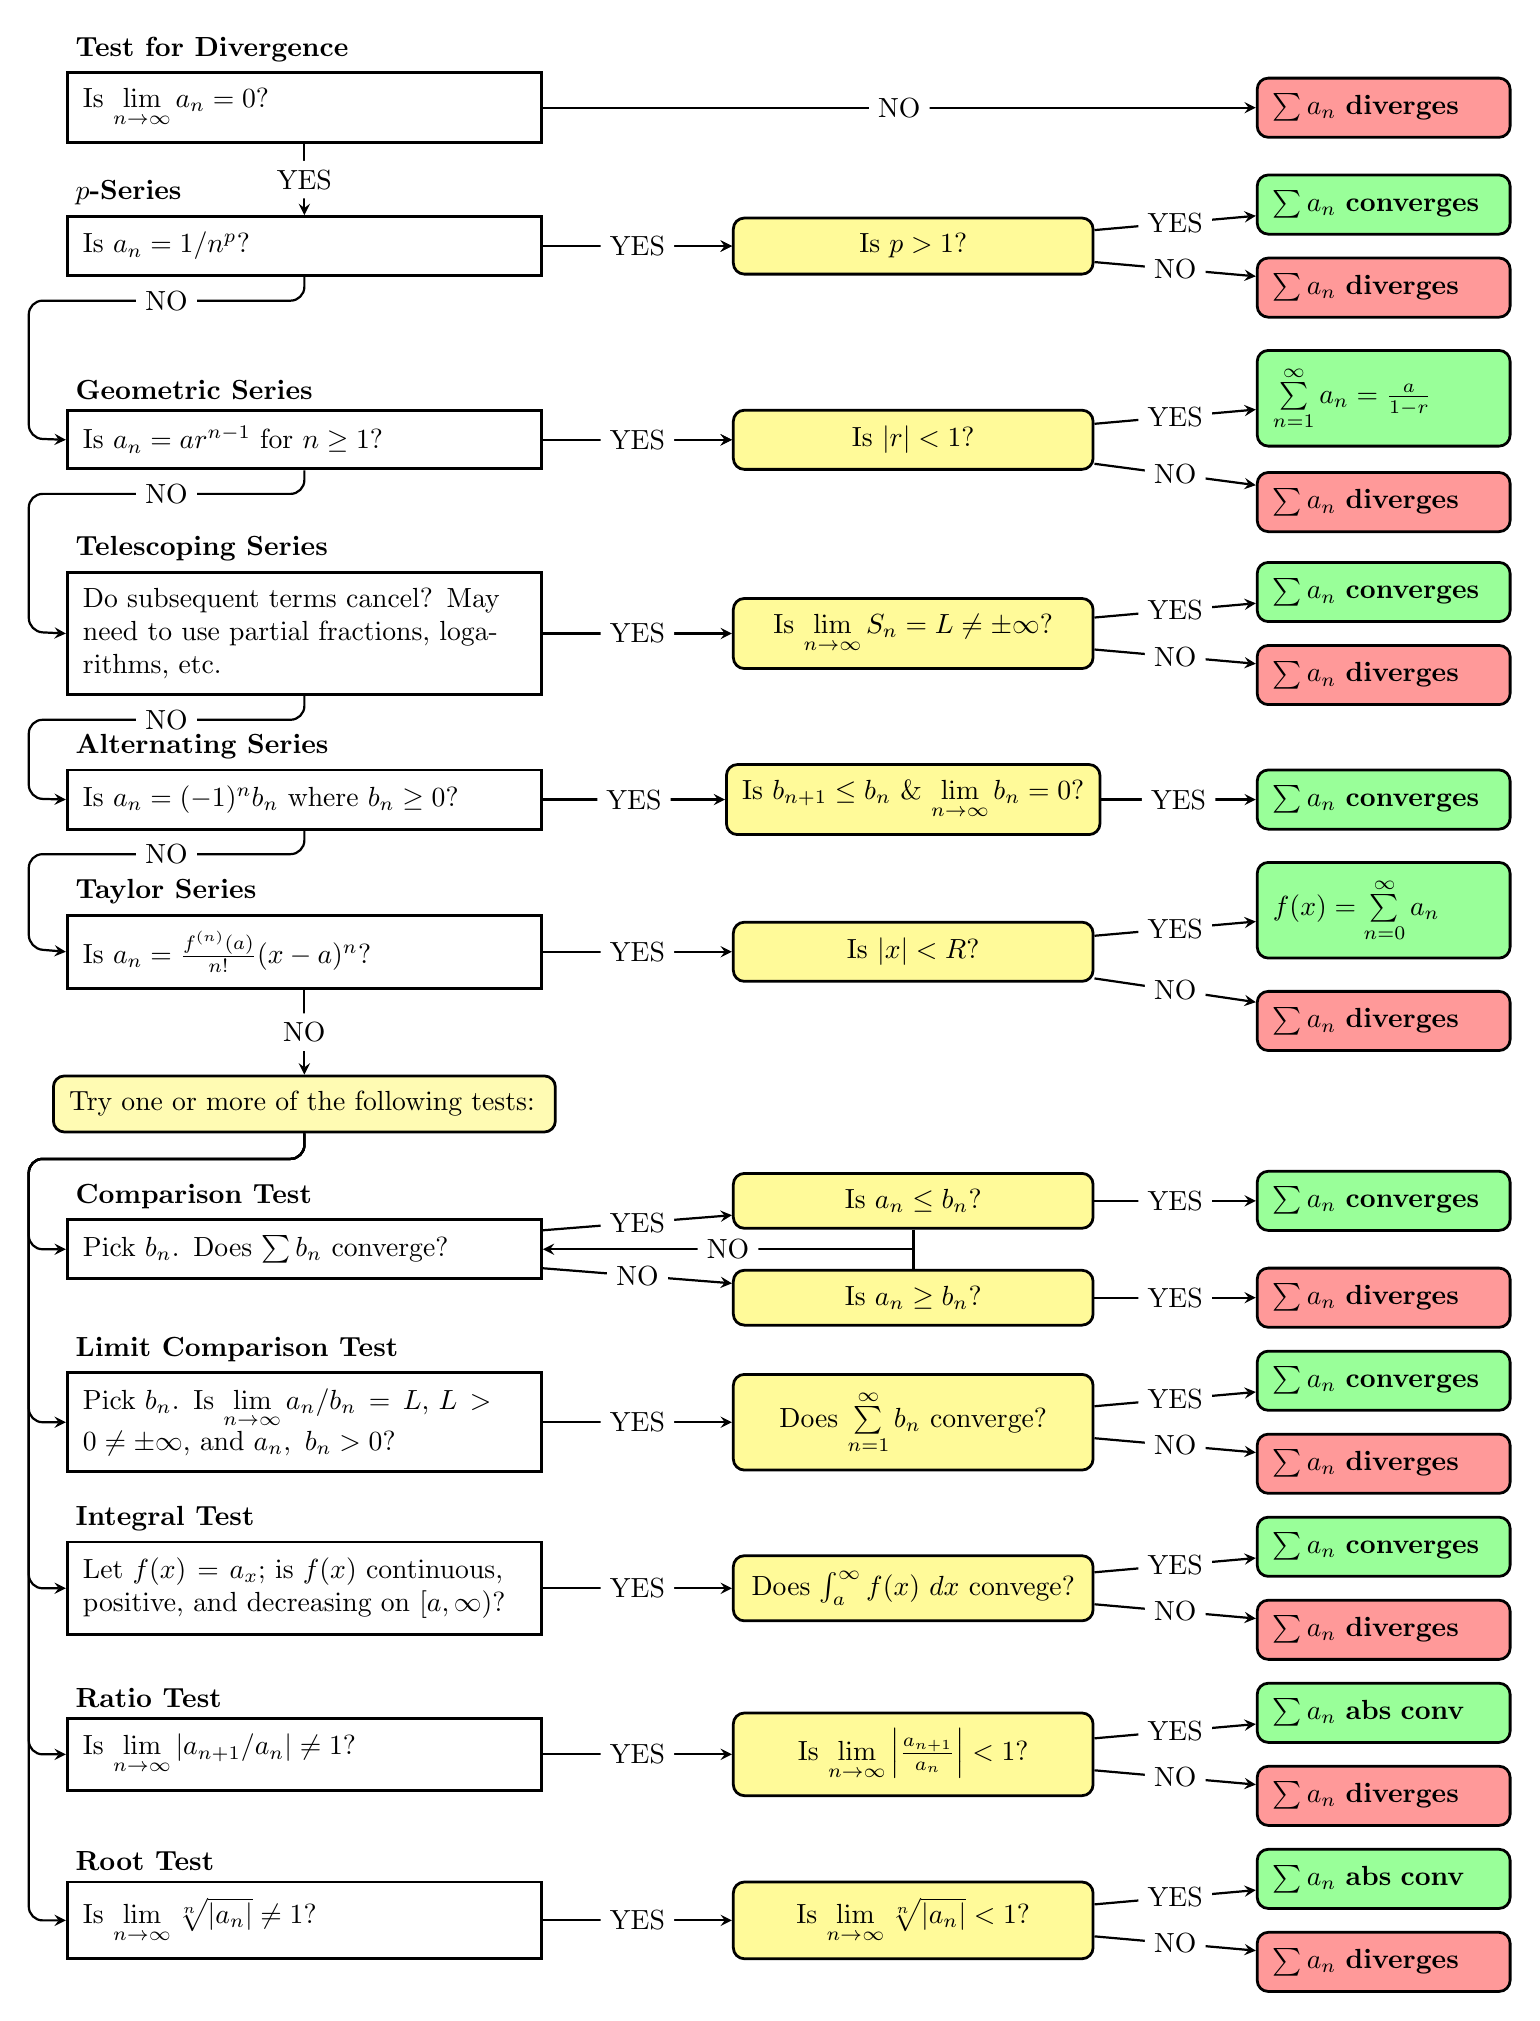
\begin{tikzpicture}[node distance=6em]
    % div test
    \node (div_test) at (0,0) [boxed, label={[anchor=south west]north west:{\textbf{Test for Divergence}}}] {Is $\lim\limits_{n \to \infty} a_n =0$?};
    \node (div_test_div) [diverges, right of=div_test] {$\sum a_n$ \textbf{diverges}};

    % p-series
    \node (p_series) [boxed, below of=div_test, label={[anchor=south west]north west:{\textbf{$p$-Series}}}, yshift=1em] {Is $a_n = 1/n^p$?};
    \node (p_series_conv) [converges, right of=p_series, yshift=1.5em] {$\sum a_n$ \textbf{converges}};
    \node (p_series_div) [diverges, right of=p_series, yshift=-1.5em] {$\sum a_n$ \textbf{diverges}};

    % geometric series
    \node (geom_series) [boxed, below of=p_series, label={[anchor=south west]north west:{\textbf{Geometric Series}}}, yshift=-1em] {Is $a_n = ar^{n-1}$ for $n \geq 1$?};
    \node (geom_series_conv) [converges, right of=geom_series, yshift=1.5em] {$\sum\limits_{n=1}^\infty a_n = \frac{a}{1-r}$};
    \node (geom_series_div) [diverges, right of=geom_series, yshift=-2.25em] {$\sum a_n$ \textbf{diverges}};

    % telescoping series
    \node (tele_series) [boxed, below of=geom_series, label={[anchor=south west]north west:{\textbf{Telescoping Series}}}, yshift=-1em] {Do subsequent terms cancel? May need to use partial fractions, logarithms, etc.};
    \node (tele_series_conv) [converges, right of=tele_series, yshift=1.5em] {$\sum a_n$ \textbf{converges}};
    \node (tele_series_div) [diverges, right of=tele_series, yshift=-1.5em] {$\sum a_n$ \textbf{diverges}};

    % alternating series
    \node (alt_series) [boxed, below of=tele_series, label={[anchor=south west]north west:{\textbf{Alternating Series}}}] {Is $a_n = (-1)^n b_n$ where $b_n \geq 0$?};
    \node (alt_series_conv) [converges, right of = alt_series] {$\sum a_n$ \textbf{converges}};

    % taylor series
    \node (taylor_series) [boxed, below of=alt_series, label={[anchor=south west]north west:{\textbf{Taylor Series}}}, yshift=0.5em] {Is $a_n = \frac{f^{(n)}(a)}{n!} (x-a)^n$?};
    \node (taylor_series_conv) [converges, right of=taylor_series, yshift=1.5em] {$f(x) = \sum\limits_{n=0}^\infty a_n$};
    \node (taylor_series_div) [diverges, right of=taylor_series, yshift=-2.5em] {$\sum a_n$ \textbf{diverges}};

    % try
    \node (try) [boxed, below of=taylor_series, text width=17em, rounded corners, yshift=0.5em, fill=yellow!30] {Try one or more of the following tests:};

    % comparison test
    \node (comp_test) [boxed, below of=try, label={[anchor=south west]north west:{\textbf{Comparison Test}}}, yshift=1em, yshift=-0.25em] {Pick ${b_n}$. Does $\sum b_n$ converge?};
    \node (comp_test_conv) [converges, right of=comp_test, yshift=1.75em] {$\sum a_n$ \textbf{converges}};
    \node (comp_test_conv2) [diverges, right of=comp_test, yshift=-1.75em] {$\sum a_n$ \textbf{diverges}};

    % limit comparison test
    \node (lim_comp_test) [boxed, below of=comp_test, label={[anchor=south west]north west:{\textbf{Limit Comparison Test}}}, yshift=-0.25em] {Pick ${b_n}$. Is $\lim\limits_{n \to \infty} a_n / b_n = L$, $L > 0 \neq \pm \infty$, and $a_n,\ b_n > 0$?};
    \node (lim_comp_test_conv) [converges, right of=lim_comp_test, yshift=1.5em] {$\sum a_n$ \textbf{converges}};
    \node (lim_comp_test_div) [diverges, right of=lim_comp_test, yshift=-1.5em] {$\sum a_n$ \textbf{diverges}};

    % integral test
    \node (integral_test) [boxed, below of=lim_comp_test, label={[anchor=south west]north west:{\textbf{Integral Test}}}] {Let $f(x) = a_x$; is $f(x)$ continuous, positive, and decreasing on $[a, \infty)$?};
    \node (integral_test_conv) [converges, right of=integral_test, yshift=1.5em] {$\sum a_n$ \textbf{converges}};
    \node (integral_test_div) [diverges, right of=integral_test, yshift=-1.5em] {$\sum a_n$ \textbf{diverges}};

    % ratio test
    \node (ratio_test) [boxed, below of=integral_test, label={[anchor=south west]north west:{\textbf{Ratio Test}}}] {Is $\lim\limits_{n \to \infty} |a_{n+1}/a_n| \neq 1$?};
    \node (ratio_test_conv) [converges, right of=ratio_test, yshift=1.5em] {$\sum a_n$ \textbf{abs conv}};
    \node (ratio_test_div) [diverges, right of=ratio_test, yshift=-1.5em] {$\sum a_n$ \textbf{diverges}};

    % root test
    \node (root_test) [boxed, below of=ratio_test, label={[anchor=south west]north west:{\textbf{Root Test}}}] {Is $\lim\limits_{n \to \infty} \sqrt[n]{|a_n|} \neq 1$?};
    \node (root_test_conv) [converges, right of=root_test, yshift=1.5em] {$\sum a_n$ \textbf{abs conv}};
    \node (root_test_div) [diverges, right of=root_test, yshift=-1.5em] {$\sum a_n$ \textbf{diverges}};


    % decisions
    \node (p_dec) [decision, right of=p_series] {Is $p > 1?$};
    \node (geom_dec) [decision, right of=geom_series] {Is $|r| < 1?$};
    \node (tele_dec) [decision, right of=tele_series] {Is $\lim\limits_{n \to \infty} S_n = L \neq \pm \infty$?};
    \node (alt_dec) [decision, right of=alt_series] {Is $b_{n+1} \leq b_n$ \& $\lim\limits_{n \to \infty} b_n = 0$?};
    \node (taylor_dec) [decision, right of=taylor_series] {Is $|x| < R$?};
    \node (comp_dec) [decision, right of=comp_test, yshift=1.75em] {Is $a_n \leq b_n$?};
    \node (comp_dec2) [decision, right of=comp_test, yshift=-1.75em] {Is $a_n \geq b_n$?};
    \node (lim_comp_dec) [decision, right of=lim_comp_test] {Does $\sum\limits_{n=1}^\infty b_n$ converge?};
    \node (integral_dec) [decision, right of=integral_test] {Does $\int_a^\infty f(x)\  dx$ convege?};
    \node (ratio_dec) [decision, right of=ratio_test] {Is $\lim\limits_{n \to \infty} \left| \frac{a_{n+1}}{a_n} \right| < 1$?};
    \node (root_dec) [decision, right of=root_test] {Is $\lim\limits_{n \to \infty} \sqrt[n]{|a_n|} < 1$?};


    % arrows
    \draw [arrow] (div_test) -- node[midway, fill=white] {NO} (div_test_div);
    \draw [arrow] (div_test) -- node[midway, fill=white] {YES} (p_series);

    \draw [arrow] (p_series) -- (p_dec);
    \draw [arrow] (p_series) -- node[midway, fill=white] {YES} (p_dec);
    \draw [arrow] (p_dec) -- node[midway, fill=white] {YES} (p_series_conv);
    \draw [arrow] (p_dec) -- node[midway, fill=white] {NO} (p_series_div);
    \draw [arrow] (p_series.south) -- +(0, -0.3) -- node[midway, fill=white] {NO} +(-3.5, -0.3) -- +(-3.5, -2.05) -- (geom_series.west);

    \draw [arrow] (geom_series) -- (geom_dec);
    \draw [arrow] (geom_series) -- node[midway, fill=white] {YES} (geom_dec);
    \draw [arrow] (geom_dec) -- node[midway, fill=white] {YES} (geom_series_conv);
    \draw [arrow] (geom_dec) -- node[midway, fill=white] {NO} (geom_series_div);
    \draw [arrow] (geom_series.south) -- +(0, -0.3) -- node[midway, fill=white] {NO} +(-3.5, -0.3) -- +(-3.5, -2.05) -- (tele_series.west);

    \draw [arrow] (tele_series) -- node[midway, fill=white] {YES} (tele_dec);
    \draw [arrow] (tele_dec) -- node[midway, fill=white] {YES} (tele_series_conv);
    \draw [arrow] (tele_dec) -- node[midway, fill=white] {NO} (tele_series_div);
    \draw [arrow] (tele_series.south) -- +(0, -0.3) -- node[midway, fill=white] {NO} +(-3.5, -0.3) -- +(-3.5, -1.3) -- (alt_series.west);

    \draw [arrow] (alt_series) -- node[midway, fill=white] {YES} (alt_dec);
    \draw [arrow] (alt_dec) -- node[midway, fill=white] {YES} (alt_series_conv);
    \draw [arrow] (alt_series.south) -- +(0, -0.3) -- node[midway, fill=white] {NO} +(-3.5, -0.3) -- +(-3.5, -1.5) -- (taylor_series.west);

    \draw [arrow] (taylor_series) -- node[midway, fill=white] {YES} (taylor_dec);
    \draw [arrow] (taylor_dec) -- node[midway, fill=white] {YES} (taylor_series_conv);
    \draw [arrow] (taylor_dec) -- node[midway, fill=white] {NO} (taylor_series_div);
    \draw [arrow] (taylor_series) -- node[midway, fill=white] {NO} (try);

    \draw [arrow] (comp_test) -- node[midway, fill=white] {YES} (comp_dec);
    \draw [arrow] (comp_test) -- node[midway, fill=white] {NO} (comp_dec2);
    \draw [arrow] (comp_dec) -- node[midway, fill=white] {YES} (comp_test_conv);
    \draw [arrow] (comp_dec2) -- node[midway, fill=white] {YES} (comp_test_conv2);

    \draw [line width=1pt] (comp_dec.south) -- coordinate (mid_pnt_comp_test) (comp_dec2.north);
    \draw [arrow] (mid_pnt_comp_test) -- node[midway, fill=white] {NO} (comp_test);

    \draw [arrow] (lim_comp_test) -- node[midway, fill=white] {YES} (lim_comp_dec);
    \draw [arrow] (lim_comp_dec) -- node[midway, fill=white] {YES} (lim_comp_test_conv);
    \draw [arrow] (lim_comp_dec) -- node[midway, fill=white] {NO} (lim_comp_test_div);

    \draw [arrow] (integral_test) -- node[midway, fill=white] {YES} (integral_dec);
    \draw [arrow] (integral_dec) -- node[midway, fill=white] {YES} (integral_test_conv);
    \draw [arrow] (integral_dec) -- node[midway, fill=white] {NO} (integral_test_div);

    \draw [arrow] (ratio_test) -- node[midway, fill=white] {YES} (ratio_dec);
    \draw [arrow] (ratio_dec) -- node[midway, fill=white] {YES} (ratio_test_conv);
    \draw [arrow] (ratio_dec) -- node[midway, fill=white] {NO} (ratio_test_div);

    \draw [arrow] (root_test) -- node[midway, fill=white] {YES} (root_dec);
    \draw [arrow] (root_dec) -- node[midway, fill=white] {YES} (root_test_conv);
    \draw [arrow] (root_dec) -- node[midway, fill=white] {NO} (root_test_div);

    % path
    \path (try.south) -- (ratio_test.west);
    \draw [arrow] (try.south) -- (0, -13.35) -- (-3.5, -13.35) |- (comp_test);
    \draw [arrow] (try.south) -- (0, -13.35) -- (-3.5, -13.35) |- (lim_comp_test);
    \draw [arrow] (try.south) -- (0, -13.35) -- (-3.5, -13.35) |- (integral_test);
    \draw [arrow] (try.south) -- (0, -13.35) -- (-3.5, -13.35) |- (root_test);
    \draw [arrow] (try.south) -- (0, -13.35) -- (-3.5, -13.35) |- (ratio_test);
\end{tikzpicture}

\end{document}
